\documentclass[11pt,a4paper]{report}
\usepackage[textwidth=37em,vmargin=30mm]{geometry}
\usepackage{calc,xunicode,amsmath,amssymb,paralist,enumitem,tabu,booktabs,datetime2,xeCJK,xeCJKfntef,listings}
\usepackage{tocloft,fancyhdr,tcolorbox,xcolor,graphicx,eso-pic,xltxtra,xelatexemoji}

\newcommand{\envyear}[0]{2025}
\newcommand{\envdatestr}[0]{2025-06-04}
\newcommand{\envfinaldir}[0]{webdb/2025/20250604/final}

\usepackage[hidelinks]{hyperref}
\hypersetup{
    colorlinks=false,
    pdfpagemode=FullScreen,
    pdftitle={Web Digest - \envdatestr}
}

\setlength{\cftbeforechapskip}{10pt}
\renewcommand{\cftchapfont}{\rmfamily\bfseries\large\raggedright}
\setlength{\cftbeforesecskip}{2pt}
\renewcommand{\cftsecfont}{\sffamily\small\raggedright}

\setdefaultleftmargin{2em}{2em}{1em}{1em}{1em}{1em}

\usepackage{xeCJK,xeCJKfntef}
\xeCJKsetup{PunctStyle=plain,RubberPunctSkip=false,CJKglue=\strut\hskip 0pt plus 0.1em minus 0.05em,CJKecglue=\strut\hskip 0.22em plus 0.2em}
\XeTeXlinebreaklocale "zh"
\XeTeXlinebreakskip = 0pt


\setmainfont{Brygada 1918}
\setromanfont{Brygada 1918}
\setsansfont{IBM Plex Sans}
\setmonofont{JetBrains Mono NL}
\setCJKmainfont{Noto Serif CJK SC}
\setCJKromanfont{Noto Serif CJK SC}
\setCJKsansfont{Noto Sans CJK SC}
\setCJKmonofont{Noto Sans CJK SC}

\setlength{\parindent}{0pt}
\setlength{\parskip}{8pt}
\linespread{1.15}

\lstset{
	basicstyle=\ttfamily\footnotesize,
	numbersep=5pt,
	backgroundcolor=\color{black!5},
	showspaces=false,
	showstringspaces=false,
	showtabs=false,
	tabsize=2,
	captionpos=b,
	breaklines=true,
	breakatwhitespace=true,
	breakautoindent=true,
	linewidth=\textwidth
}






\newcommand{\coverpic}[2]{
    % argv: itemurl, authorname
    Cover photo by #2~~(\href{#1}{#1})
}
\newcommand{\makeheader}[0]{
    \begin{titlepage}
        % \newgeometry{hmargin=15mm,tmargin=21mm,bmargin=12mm}
        \begin{center}
            
            \rmfamily\scshape
            \fontspec{BaskervilleF}
            \fontspec{Old Standard}
            \fontsize{59pt}{70pt}\selectfont
            WEB\hfill DIGEST
            
            \vfill
            % \vskip 30pt
            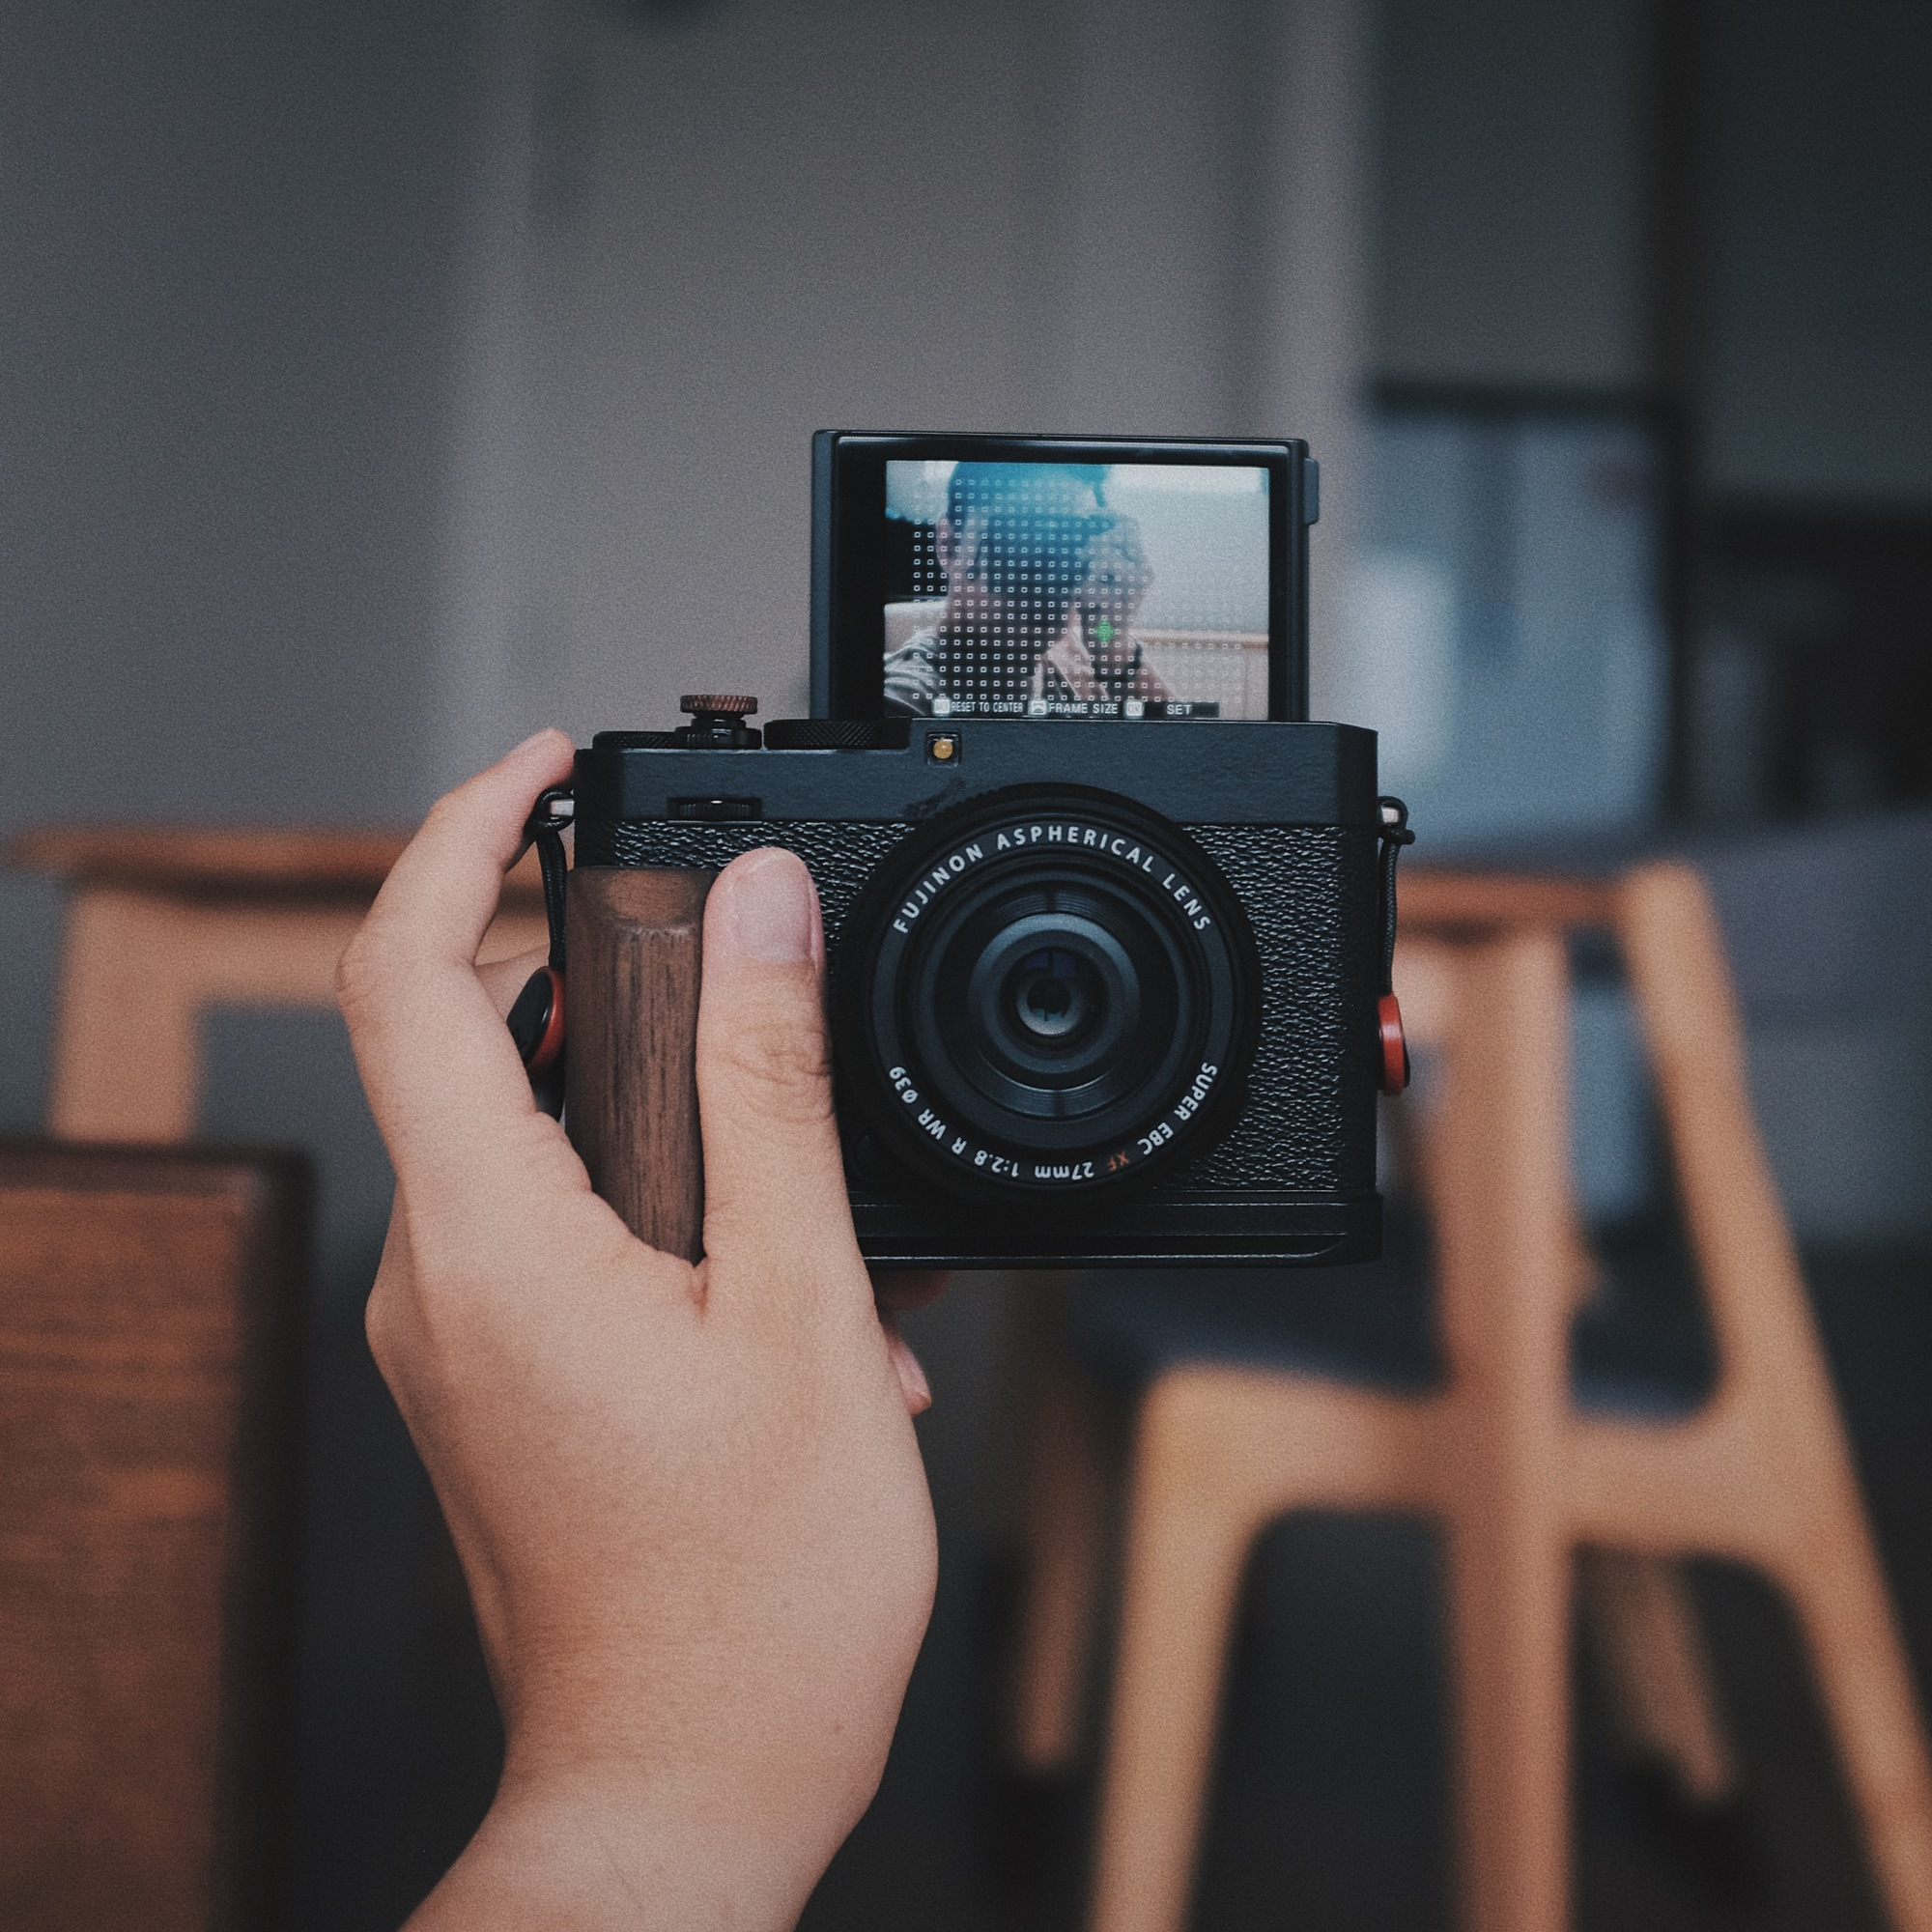
\includegraphics[width=\linewidth]{\envfinaldir/coverpic-prod.jpg}\par
            % \vskip 30pt
            \vfill

            \normalsize\rmfamily\scshape
            \copyright{} The Web Digest Project \hfill\large \envdatestr
        \end{center}
    \end{titlepage}
    % \restoregeometry
}
\newcommand{\simplehref}[1]{%
    \textcolor{blue!80!green}{\href{#1}{#1}}%
}
\renewcommand{\contentsname}{\center\Huge\sffamily\bfseries Contents\par\vskip 20pt}
\newcounter{ipartcounter}
\setcounter{ipartcounter}{0}
\newcommand{\ipart}[1]{
    % \vskip 20pt
    \clearpage
    \stepcounter{ipartcounter}
    \phantomsection
    \addcontentsline{toc}{chapter}{#1}
    % \begin{center}
    %     \Huge
    %     \sffamily\bfseries
    %     #1
    % \end{center}
    % \vskip 20pt plus 7pt
}
\newcounter{ichaptercounter}
\setcounter{ichaptercounter}{0}
\newcommand{\ichapter}[1]{
    % \vskip 20pt
    \clearpage
    \stepcounter{ichaptercounter}
    \phantomsection
    \addcontentsline{toc}{section}{\numberline{\arabic{ichaptercounter}}#1}
    \begin{center}
        \Huge
        \sffamily\bfseries
        #1
    \end{center}
    \vskip 20pt plus 7pt
}
\newcommand{\entrytitlefont}[1]{\subsection*{\raggedright\Large\sffamily\bfseries#1}}
\newcommand{\entryitemGeneric}[2]{
    % argv: title, url
    \parbox{\linewidth}{
        \entrytitlefont{#1}\par\vskip 5pt
        \footnotesize\ttfamily\mdseries
        \simplehref{#2}
    }\vskip 11pt plus 11pt minus 1pt
}
\newcommand{\entryitemGithub}[3]{
    % argv: title, url, desc
    \parbox{\linewidth}{
        \entrytitlefont{#1}\par\vskip 5pt
        \footnotesize\ttfamily\mdseries
        \simplehref{#2}\par\vskip 5pt
        \small\rmfamily\mdseries#3
    }\vskip 11pt plus 11pt minus 1pt
}
\newcommand{\entryitemAp}[3]{
    % argv: title, url, desc
    \parbox{\linewidth}{
        \entrytitlefont{#1}\par\vskip 5pt
        \footnotesize\ttfamily\mdseries
        \simplehref{#2}\par\vskip 5pt
        \small\rmfamily\mdseries#3
    }\vskip 11pt plus 11pt minus 1pt
}
\newcommand{\entryitemHackernews}[3]{
    % argv: title, hnurl, rawurl
    % \parbox{\linewidth}{
    %     \entrytitlefont{#1}\par\vskip 5pt
    %     \footnotesize\ttfamily\mdseries
    %     \simplehref{#3}\par
    %     \textcolor{black!50}{\href{#2}{#2}}
    % }\vskip 11pt plus 11pt minus 1pt
    \begin{minipage}{\linewidth}
            \entrytitlefont{#1}\par\vskip 5pt
            \footnotesize\ttfamily\mdseries
            \simplehref{#3}\par
            \textcolor{black!50}{\href{#2}{#2}}
    \end{minipage}\par\vskip 11pt plus 11pt minus 1pt
}







\begin{document}

\makeheader

\tableofcontents\clearpage




\ipart{Developers}
\ichapter{Hacker News}
\entryitemTwoLinks{Deep learning gets the glory, deep fact checking gets ignored}{https://news.ycombinator.com/item?id=44174965}{https://rachel.fast.ai/posts/2025-06-04-enzyme-ml-fails/index.html}

\entryitemTwoLinks{Show HN: AirAP AirPlay server - AirPlay to an iOS Device}{https://news.ycombinator.com/item?id=44174190}{https://github.com/neon443/AirAP}

\entryitemTwoLinks{Swift at Apple: Migrating the Password Monitoring Service from Java}{https://news.ycombinator.com/item?id=44172166}{https://www.swift.org/blog/swift-at-apple-migrating-the-password-monitoring-service-from-java/}

\entryitemTwoLinks{(On | No) Syntactic Support for Error Handling}{https://news.ycombinator.com/item?id=44171677}{https://go.dev/blog/error-syntax}

\entryitemTwoLinks{The Small World of English}{https://news.ycombinator.com/item?id=44170968}{https://www.inotherwords.app/linguabase/}

\entryitemTwoLinks{Claude Code Is My Computer}{https://news.ycombinator.com/item?id=44170967}{https://steipete.me/posts/2025/claude-code-is-my-computer}

\entryitemTwoLinks{Builder.ai Collapses: \$1.5B 'AI' Startup Exposed as 'Indians'}{https://news.ycombinator.com/item?id=44169759}{https://www.ibtimes.co.uk/builderai-collapses-15bn-ai-startup-exposed-actually-indians-pretending-bots-1734784}

\entryitemTwoLinks{Vision Language Models Are Biased}{https://news.ycombinator.com/item?id=44169413}{https://vlmsarebiased.github.io/}

\entryitemTwoLinks{Covert Web-to-App Tracking via Localhost on Android}{https://news.ycombinator.com/item?id=44169314}{https://localmess.github.io/}

\entryitemTwoLinks{Show HN: I wrote a Java decompiler in pure C language}{https://news.ycombinator.com/item?id=44169132}{https://github.com/neocanable/garlic}

\entryitemTwoLinks{Covert Web-to-App Tracking via Localhost on Android}{https://news.ycombinator.com/item?id=44169115}{https://localmess.github.io/}

\entryitemTwoLinks{NYC Drivers Who Run Red Lights Get Tickets. E-Bike Riders Get Court Dates}{https://news.ycombinator.com/item?id=44169050}{https://www.nytimes.com/2025/05/24/nyregion/ebikes-scooters-cyclists-nyc.html}

\entryitemTwoLinks{How Ukraine's killer drones are beating Russian jamming}{https://news.ycombinator.com/item?id=44168658}{https://spectrum.ieee.org/ukraine-killer-drones}

\entryitemTwoLinks{EU Commission refuses to disclose authors behind its mass surveillance proposal}{https://news.ycombinator.com/item?id=44168134}{https://old.reddit.com/r/europe/comments/1l2655n/the\_eu\_commission\_refuses\_to\_disclose\_the/}

\entryitemTwoLinks{Quarkdown: A modern Markdown-based typesetting system}{https://news.ycombinator.com/item?id=44167592}{https://github.com/iamgio/quarkdown}

\entryitemTwoLinks{The Metamorphosis of Prime Intellect (1994)}{https://news.ycombinator.com/item?id=44166155}{https://localroger.com/prime-intellect/mopiall.html}

\entryitemTwoLinks{AI makes the humanities more important, but also weirder}{https://news.ycombinator.com/item?id=44166102}{https://resobscura.substack.com/p/ai-makes-the-humanities-more-important}

\entryitemTwoLinks{Conformance checking at MongoDB: Testing that our code matches our TLA+ specs}{https://news.ycombinator.com/item?id=44163496}{https://www.mongodb.com/blog/post/engineering/conformance-checking-at-mongodb-testing-our-code-matches-our-tla-specs}

\entryitemTwoLinks{Japanese scientists develop artificial blood compatible with all blood types}{https://news.ycombinator.com/item?id=44163428}{https://www.tokyoweekender.com/entertainment/tech-trends/japanese-scientists-develop-artificial-blood/}

\entryitemTwoLinks{My AI skeptic friends are all nuts}{https://news.ycombinator.com/item?id=44163063}{https://fly.io/blog/youre-all-nuts/}\ichapter{Phoronix}
\entryitemGeneric{\hskip 0pt{}Linux 6.16 Merges Support For The Apple Magic Mouse 2 USB-C}{https://www.phoronix.com/news/Linux-6.16-HID}

\entryitemGeneric{\hskip 0pt{}Linux 6.16 Brings Many Laptop Driver Improvements, New Dasharo ACPI Driver}{https://www.phoronix.com/news/Linux-6.16-Platform-Drivers-x86}

\entryitemGeneric{\hskip 0pt{}SMT Proves Very Advantageous For AMD Ryzen AI MAX Strix Halo Performance}{https://www.phoronix.com/review/amd-strix-halo-smt}

\entryitemGeneric{\hskip 0pt{}AMD Upstreams Efficient Malloc Support On GPUs For LLVM libc}{https://www.phoronix.com/news/LLVM-libc-GPU-malloc-Upstream}

\entryitemGeneric{\hskip 0pt{}ByoWave Modular Proteus Controller Kit Support Lands In Linux 6.16}{https://www.phoronix.com/news/Linux-6.16-Input}

\entryitemGeneric{\hskip 0pt{}NVMe FDP Block Write Streams, IO\_uring DMA-BUF Zero Copy Receive Land In Linux 6.16}{https://www.phoronix.com/news/Linux-6.16-Block-IO\_uring}

\entryitemGeneric{\hskip 0pt{}FUSE Improvements Merged For Linux 6.16 To Enhance File-Systems In User-Space}{https://www.phoronix.com/news/Linux-6.16-FUSE}

\entryitemGeneric{\hskip 0pt{}Phoronix Turns 21 This Week - Show Your Support For Linux Hardware Reviews}{https://www.phoronix.com/news/Phoronix-21-Birthday-Premium}

\entryitemGeneric{\hskip 0pt{}New Rust Abstractions Added In Linux 6.16 For More Core Areas}{https://www.phoronix.com/news/Linux-6.16-More-Rust-Core}\ichapter{Dribbble}
\entryitemGeneric{\hskip 0pt{}Aquasan}{https://dribbble.com/shots/26100535-Aquasan}

\entryitemGeneric{\hskip 0pt{}Eagle}{https://dribbble.com/shots/26099428-Eagle}

\entryitemGeneric{\hskip 0pt{}Mnp Technologies - Logo Design}{https://dribbble.com/shots/26092034-Mnp-Technologies-Logo-Design}

\entryitemGeneric{\hskip 0pt{}Singular Logo Concept (Unused)}{https://dribbble.com/shots/26091755-Singular-Logo-Concept-Unused}

\entryitemGeneric{\hskip 0pt{}Cre8tera // Website}{https://dribbble.com/shots/26091009-Cre8tera-Website}

\entryitemGeneric{\hskip 0pt{}Cool Pool Logo Design - Letter C Monogram}{https://dribbble.com/shots/26091401-Cool-Pool-Logo-Design-Letter-C-Monogram}

\entryitemGeneric{\hskip 0pt{}Gorilla + Bar Chart Logo}{https://dribbble.com/shots/26092670-Gorilla-Bar-Chart-Logo}

\entryitemGeneric{\hskip 0pt{}zeero logo design}{https://dribbble.com/shots/26087342-zeero-logo-design}

\entryitemGeneric{\hskip 0pt{}Create email inbox composition}{https://dribbble.com/shots/26083118-Create-email-inbox-composition}

\entryitemGeneric{\hskip 0pt{}Shori Brand}{https://dribbble.com/shots/26088139-Shori-Brand}

\entryitemGeneric{\hskip 0pt{}Roaring Bear}{https://dribbble.com/shots/26087788-Roaring-Bear}

\entryitemGeneric{\hskip 0pt{}Eagle}{https://dribbble.com/shots/26085536-Eagle}

\entryitemGeneric{\hskip 0pt{}Hand-drawn illustration pack}{https://dribbble.com/shots/26084735-Hand-drawn-illustration-pack}

\entryitemGeneric{\hskip 0pt{}Dog Mascot Various Poses}{https://dribbble.com/shots/26087977-Dog-Mascot-Various-Poses}

\entryitemGeneric{\hskip 0pt{}Branding Concept for Europe}{https://dribbble.com/shots/26087652-Branding-Concept-for-Europe}

\entryitemGeneric{\hskip 0pt{}B2B Dashboard \& Web App UI UX Design for Carbon Solutions}{https://dribbble.com/shots/26076624-B2B-Dashboard-Web-App-UI-UX-Design-for-Carbon-Solutions}

\entryitemGeneric{\hskip 0pt{}Patriot Logo Design (Unused for Sale)}{https://dribbble.com/shots/26081047-Patriot-Logo-Design-Unused-for-Sale}

\entryitemGeneric{\hskip 0pt{}Heliopoint}{https://dribbble.com/shots/26081987-Heliopoint}

\entryitemGeneric{\hskip 0pt{}Apple}{https://dribbble.com/shots/26084067-Apple}

\entryitemGeneric{\hskip 0pt{}Illustration}{https://dribbble.com/shots/26083223-Illustration}

\entryitemGeneric{\hskip 0pt{}Europe Logo Animation}{https://dribbble.com/shots/26082596-Europe-Logo-Animation}

\entryitemGeneric{\hskip 0pt{}Arc Logo}{https://dribbble.com/shots/26083648-Arc-Logo}

\entryitemGeneric{\hskip 0pt{}Heyo Turns 2!}{https://dribbble.com/shots/26078572-Heyo-Turns-2}

\entryitemGeneric{\hskip 0pt{}Fox Brand Mascot}{https://dribbble.com/shots/26077954-Fox-Brand-Mascot}


\ipart{Developers~~~~(zh-Hans)}
\ichapter{Solidot}
\entryitemGeneric{\hskip 0pt{}报告称 AI 的普及和增长``史无前例''}{https://www.solidot.org/story?sid=81457}

\entryitemGeneric{\hskip 0pt{}仙女座和银河系未必会相撞}{https://www.solidot.org/story?sid=81456}

\entryitemGeneric{\hskip 0pt{}锻炼能显著降低结肠癌的复发和死亡风险}{https://www.solidot.org/story?sid=81455}

\entryitemGeneric{\hskip 0pt{}微软对 Windows 11 设备强制统一 USB-C 功能}{https://www.solidot.org/story?sid=81454}

\entryitemGeneric{\hskip 0pt{}Stack Overflow 的衰落始于其声誉系统}{https://www.solidot.org/story?sid=81453}

\entryitemGeneric{\hskip 0pt{}中国出现假装上班的新商业模式}{https://www.solidot.org/story?sid=81452}

\entryitemGeneric{\hskip 0pt{}微软 Google 等将统一国家支持的黑客组织的绰号}{https://www.solidot.org/story?sid=81451}

\entryitemGeneric{\hskip 0pt{}美国部分 incel 选择躺平}{https://www.solidot.org/story?sid=81450}

\entryitemGeneric{\hskip 0pt{}朝鲜智能手机会自动替换禁词每 5 分钟截屏}{https://www.solidot.org/story?sid=81449}

\entryitemGeneric{\hskip 0pt{}我国科学家构建 300 公里级量子直接通信网络}{https://www.solidot.org/story?sid=81448}

\entryitemGeneric{\hskip 0pt{}M8.2 级太阳耀斑引发 G4 级地磁风暴}{https://www.solidot.org/story?sid=81447}

\entryitemGeneric{\hskip 0pt{}美国的加密货币战略储备规模有多大}{https://www.solidot.org/story?sid=81446}

\entryitemGeneric{\hskip 0pt{}俄罗斯公共采购数据库泄漏核基地细节}{https://www.solidot.org/story?sid=81445}

\entryitemGeneric{\hskip 0pt{}黑猩猩将敲击树干作为一种交流模式}{https://www.solidot.org/story?sid=81444}

\entryitemGeneric{\hskip 0pt{}美国科技公司减少招聘应届生}{https://www.solidot.org/story?sid=81443}

\entryitemGeneric{\hskip 0pt{}AI 耗电量预计将在年底超过比特币}{https://www.solidot.org/story?sid=81442}

\entryitemGeneric{\hskip 0pt{}NASA 卫星确认火星溅射的证据}{https://www.solidot.org/story?sid=81441}

\entryitemGeneric{\hskip 0pt{}世界面临新形式的气候否认——经济不可行}{https://www.solidot.org/story?sid=81440}\ichapter{V2EX}
\entryitemGeneric{\hskip 0pt{}[问与答] 有没有大佬有兴趣对这个 整站下载 破解软件 Offline Explorer 分析一下 里面的病毒?}{https://www.v2ex.com/t/1136178}

\entryitemGeneric{\hskip 0pt{}[远程工作] [远程工作] 聚合支付平台招开发(SpringCloud/Dubbo+Vue),有客户、有业务,寻找合拍团队小伙伴(前后端全栈开发优先) 项目负责人 Bènją ✈️ @birn\_bles\_dord}{https://www.v2ex.com/t/1136177}

\entryitemGeneric{\hskip 0pt{}[分享发现] 解决使用小米换机后功耗变大、发热。}{https://www.v2ex.com/t/1136175}

\entryitemGeneric{\hskip 0pt{}[远程工作] [Remote] [Full-time] Product Manager – Web3 \& DeFi}{https://www.v2ex.com/t/1136174}

\entryitemGeneric{\hskip 0pt{}[问与答] 有什么好用的 整站下载 工具吗?}{https://www.v2ex.com/t/1136173}

\entryitemGeneric{\hskip 0pt{}[问与答] 想不起一个有大模型性价比图的网站}{https://www.v2ex.com/t/1136172}

\entryitemGeneric{\hskip 0pt{}[问与答] 大模型的 api 为什么设计成无状态的?}{https://www.v2ex.com/t/1136171}

\entryitemGeneric{\hskip 0pt{}[问与答] 谈一谈我中学时期因吃辣条被举报导致被老师扇耳光的经历}{https://www.v2ex.com/t/1136170}

\entryitemGeneric{\hskip 0pt{}[天黑以后] [记录]-2025-06-04 成长与收敛的关系 (AI 生成)}{https://www.v2ex.com/t/1136169}

\entryitemGeneric{\hskip 0pt{}[问与答] 后端开发第一次装机,听劝}{https://www.v2ex.com/t/1136168}

\entryitemGeneric{\hskip 0pt{}[职场话题] Swift 岗的前景怎么样?(和 android 和前端比起来)}{https://www.v2ex.com/t/1136167}

\entryitemGeneric{\hskip 0pt{}[程序员] 我开发了一个一站式订阅各大主流开源软件 Release 的 Telegram Channel,欢迎大家 Join}{https://www.v2ex.com/t/1136166}

\entryitemGeneric{\hskip 0pt{}[问与答] 远景论坛上不去了}{https://www.v2ex.com/t/1136165}

\entryitemGeneric{\hskip 0pt{}[程序员] 推荐一款 在线 SOCKS5/HTTP 代理检测工具}{https://www.v2ex.com/t/1136164}

\entryitemGeneric{\hskip 0pt{}[全球工单系统] Brave v1.79.118 Chromium 137.0.7151.61 当在搜索栏输入文字的时候会卡死}{https://www.v2ex.com/t/1136163}

\entryitemGeneric{\hskip 0pt{}[iCloud] 京东 618 的 icloud+ 充值是不是有问题?}{https://www.v2ex.com/t/1136162}

\entryitemGeneric{\hskip 0pt{}[问与答] 听说 cursor 可以用支付宝支付了, 但是我为什么没有这个选项呢?}{https://www.v2ex.com/t/1136161}

\entryitemGeneric{\hskip 0pt{}[分享创造] 分享一个我做的多标签翻译网站,相比 Google 翻译,增加多标签+长文本翻译}{https://www.v2ex.com/t/1136157}

\entryitemGeneric{\hskip 0pt{}[职场话题] 怎么消解工作中的负面情绪和内耗?}{https://www.v2ex.com/t/1136156}

\entryitemGeneric{\hskip 0pt{}[Android] 安卓有什么好用的 pdf 软件可以复制文字的}{https://www.v2ex.com/t/1136155}

\entryitemGeneric{\hskip 0pt{}[问与答] 有没有小主机支持 128GB 内存的?}{https://www.v2ex.com/t/1136152}

\entryitemGeneric{\hskip 0pt{}[问与答] 有什么安卓二维码扫描工具能达到微信的水准}{https://www.v2ex.com/t/1136151}

\entryitemGeneric{\hskip 0pt{}[分享创造] 开源项目分享:小弟把之前写的一个增强 ast 分析体验的插件优化了一波,感兴趣的大佬可以康康哈}{https://www.v2ex.com/t/1136148}

\entryitemGeneric{\hskip 0pt{}[分享发现] 在某宝某鱼搜索``短信猫''关键字会出现普法界面}{https://www.v2ex.com/t/1136147}

\entryitemGeneric{\hskip 0pt{}[酷工作] 招聘服务员(解忧渡)}{https://www.v2ex.com/t/1136145}

\entryitemGeneric{\hskip 0pt{}[酷工作] 成都腾讯招 kubernetes 方向研发}{https://www.v2ex.com/t/1136144}

\entryitemGeneric{\hskip 0pt{}[问与答] 有点纠结:到底是换九号电动车,还是换更长续航的电池?}{https://www.v2ex.com/t/1136143}

\entryitemGeneric{\hskip 0pt{}[NAS] NAS 方案分享: 2025 年入手群晖 DS1821+}{https://www.v2ex.com/t/1136142}

\entryitemGeneric{\hskip 0pt{}[编程] 从 markdown 编辑器直接复制内容到微信公众号平台保持样式不变,这是怎么做到的?}{https://www.v2ex.com/t/1136141}

\entryitemGeneric{\hskip 0pt{}[问与答] 怎么 Cursor 只能用手机热点连接:}{https://www.v2ex.com/t/1136140}

\entryitemGeneric{\hskip 0pt{}[海外留学] 有没有集合片源的付费电视软件,长期可用的}{https://www.v2ex.com/t/1136139}

\entryitemGeneric{\hskip 0pt{}[云计算] 吐槽阿里云,把我用了十年的网站备案吊销了。。}{https://www.v2ex.com/t/1136138}

\entryitemGeneric{\hskip 0pt{}[Android] 2025 年,还有人在日常使用 pixel4 吗}{https://www.v2ex.com/t/1136137}

\entryitemGeneric{\hskip 0pt{}[酷工作] 招聘酒吧店长(解忧渡)}{https://www.v2ex.com/t/1136136}

\entryitemGeneric{\hskip 0pt{}[酷工作] [北京、上海、百万年薪] AI 剪辑公司在找 CTO}{https://www.v2ex.com/t/1136135}

\entryitemGeneric{\hskip 0pt{}[问与答] 码农如果手握 300 万是掏空买房留在大城市还是回县成养老🫠}{https://www.v2ex.com/t/1136134}

\entryitemGeneric{\hskip 0pt{}[Notion] 我写了一个 notion 插件,把微信消息转发到 notion,并且用大模型整理保存}{https://www.v2ex.com/t/1136133}

\entryitemGeneric{\hskip 0pt{}[程序员] 想开发一个新的开源软件,视频/文章一键同步多平台+多平台数据管理功能}{https://www.v2ex.com/t/1136132}

\entryitemGeneric{\hskip 0pt{}[程序员] 国内有哪些大学讲授 Lisp/Scheme/Racket?}{https://www.v2ex.com/t/1136130}

\entryitemGeneric{\hskip 0pt{}[职场话题] 在 v2 看了这么多兄弟被裁,现出现在自己身上了,汇报一下吧}{https://www.v2ex.com/t/1136129}

\entryitemGeneric{\hskip 0pt{}[汽车] 你们会不会开雾灯?}{https://www.v2ex.com/t/1136128}

\entryitemGeneric{\hskip 0pt{}[iDev] 大家的 iOS 开发者有没有遇到要求提供身份证和持股信息?不知道大家有没有遇到,最后怎么解决的?}{https://www.v2ex.com/t/1136127}

\entryitemGeneric{\hskip 0pt{}[投资] 存款 300 万该如何投资理财}{https://www.v2ex.com/t/1136126}

\entryitemGeneric{\hskip 0pt{}[分享创造] 用 cursor 写了一个 epub 阅读器。}{https://www.v2ex.com/t/1136124}

\entryitemGeneric{\hskip 0pt{}[程序员] cursor 技巧!.再也不用担心 cursor 500 次不够用了}{https://www.v2ex.com/t/1136123}

\entryitemGeneric{\hskip 0pt{}[酷工作] New /hot Job:  Job Title: HR \& Admin Generalist (Mandarin-speaking) Location: Singapore}{https://www.v2ex.com/t/1136122}

\entryitemGeneric{\hskip 0pt{}[淘宝] 分享一下近期在淘宝的糟糕售后体验}{https://www.v2ex.com/t/1136120}

\entryitemGeneric{\hskip 0pt{}[Docker] 有没有可行的 reproducible 容器环境方案?}{https://www.v2ex.com/t/1136118}

\entryitemGeneric{\hskip 0pt{}[问与答] 有没有老哥了解甘氨酸镁+维生素 B6 的组合}{https://www.v2ex.com/t/1136115}

\entryitemGeneric{\hskip 0pt{}[奇思妙想] 播客录制踩坑记录}{https://www.v2ex.com/t/1136114}


\ipart{Generic News}







\clearpage
\leavevmode\vfill
\footnotesize

Copyright \copyright{} 2023-2025 Neruthes and other contributors.

This document is published with CC BY-NC-ND 4.0 license.

The entries listed in this newsletter may be copyrighted by their respective creators.

This newsletter is generated by the Web Digest project.

The newsletters are also delivered via Telegram channel \CJKunderline{\href{https://t.me/webdigestchannel}{https://t.me/webdigestchannel}}.\\
RSS feed is available at \CJKunderline{\href{https://webdigest.pages.dev/rss.xml}{https://webdigest.pages.dev/rss.xml}}.

This newsletter is available in PDF at
\CJKunderline{\href{https://webdigest.pages.dev/}{https://webdigest.pages.dev/}}.

The source code being used to generate this newsletter is available at\\
\CJKunderline{\href{https://github.com/neruthes/webdigest}{https://github.com/neruthes/webdigest}}.

This newsletter is also available in
\CJKunderline{\href{http://webdigest.pages.dev/readhtml/\envyear/WebDigest-20250604.html}{HTML}} and
\CJKunderline{\href{https://github.com/neruthes/webdigest/blob/master/markdown/\envyear/WebDigest-20250604.md}{Markdown}}.


\coverpic{https://unsplash.com/photos/peacock-feathers-display-beautiful-intricate-patterns-4FLmDMG6wQs}{Dennis Yu}


\end{document}
